\documentclass[aspectratio=169,xcolor=table]{beamer}

\usetheme{ccc}

\usepackage{fontspec}
\usepackage{blindtext}
\usepackage{graphicx}
\usepackage{listings}
\usepackage{appendixnumberbeamer}
\usepackage{tikz}
\usepackage{pgfplots}
\usepackage{pgf-pie}
\usepackage{pifont}
\usepackage{booktabs}
\usepackage{changepage}
\usepackage{amsmath}
\usetikzlibrary{positioning}
\usetikzlibrary{arrows.meta}
\usetikzlibrary{shapes.geometric}
\usetikzlibrary{calc}
\usetikzlibrary{fit}
\usetikzlibrary{graphs}
\usetikzlibrary{matrix}
\usetikzlibrary{backgrounds}
\usepackage[backend=biber]{biblatex}

\definecolor{lightgray}{gray}{0.9}

% bright paul tol's colors
\definecolor{bBlue}{HTML}{4477AA}
\definecolor{bCyan}{HTML}{66CCEE}
\definecolor{bGreen}{HTML}{228833}
\definecolor{bYellow}{HTML}{CCBB44}
\definecolor{bRed}{HTML}{EE6677}
\definecolor{bPurple}{HTML}{AA3377}
\definecolor{bGray}{HTML}{BBBBBB}

% vibrant paul tol's colors
\definecolor{vBlue}{HTML}{0077BB}
\definecolor{vCyan}{HTML}{33BBEE}
\definecolor{vTeal}{HTML}{009988}
\definecolor{vOrange}{HTML}{EE7733}
\definecolor{vRed}{HTML}{CC3311}
\definecolor{vMagenta}{HTML}{EE3377}
\definecolor{vGray}{HTML}{BBBBBB}

% muted paul tol's colors
\definecolor{mIndigo}{HTML}{332288}
\definecolor{mCyan}{HTML}{88CCEE}
\definecolor{mTeal}{HTML}{44AA99}
\definecolor{mGreen}{HTML}{117733}
\definecolor{mOlive}{HTML}{999933}
\definecolor{mSand}{HTML}{DDCC77}
\definecolor{mRose}{HTML}{CC6677}
\definecolor{mWine}{HTML}{882255}
\definecolor{mPurple}{HTML}{AA4499}

% pale paul tol's colors
\definecolor{pBlue}{HTML}{BBCCEE}
\definecolor{pCyan}{HTML}{CCEEFF}
\definecolor{pGreen}{HTML}{CCDDAA}
\definecolor{pYellow}{HTML}{EEEEBB}
\definecolor{pRed}{HTML}{FFCCCC}
\definecolor{pGray}{HTML}{DDDDDD}

% dark paul tol's colors
\definecolor{dBlue}{HTML}{222255}
\definecolor{dCyan}{HTML}{225555}
\definecolor{dGreen}{HTML}{225522}
\definecolor{dYellow}{HTML}{666633}
\definecolor{dRed}{HTML}{663333}
\definecolor{dGray}{HTML}{555555}

% light paul tol's colors
\definecolor{lBlue}{HTML}{77AADD}
\definecolor{lCyan}{HTML}{99DDFF}
\definecolor{lMint}{HTML}{44BB99}
\definecolor{lPear}{HTML}{BBCC33}
\definecolor{lOlive}{HTML}{AAAA00}
\definecolor{lYellow}{HTML}{EEDD88}
\definecolor{lOrange}{HTML}{EE8866}
\definecolor{lPink}{HTML}{FFAABB}
\definecolor{lGray}{HTML}{DDDDDD}

\addbibresource{zotero.bib}

\DeclareCiteCommand{\fullcite}
  {\usebibmacro{prenote}}
  {\tiny\clearfield{url}%
    \clearfield{pages}%
    \clearfield{doi}%
    \clearfield{isbn}%
    \clearfield{note}%
    \clearlist{location}%
    \clearfield{date}%
    \clearfield{urlday}%
    \clearfield{urlmonth}%
    \clearfield{urlyear}%
    \iffieldundef{booktitle}{}{\clearfield{eventtitle}}%
   \clearfield{pagetotal}%
   \clearfield{edition}%
   \clearfield{labelyear}%
   \usedriver
     {\DeclareNameAlias{sortname}{default}}
     {\thefield{entrytype}}}
  {\multicitedelim}
  {\usebibmacro{postnote}}

%\setsansfont[BoldFont={Fira Sans SemiBold}]{Fira Sans Book}
\makeatletter
\newlength\beamerleftmargin
\setlength\beamerleftmargin{\Gm@lmargin}
\makeatother

\setbeamersize{text margin left=5em,text margin right=5em}

\title{Learning Vulnerability Discovery with Global-Relational Models}
\subtitle{Research Project Compiler Construction}
\author{Benno Fünfstück}
\date{October 7, 2021}

\begin{document}

%\includeonlyframes{current}

\tikzset{
  onslide/.code args={<#1>#2}{%
    \only<#1>{\pgfkeysalso{#2}}% \pgfkeysalso doesn't change the path
  },
  temporal/.code args={<#1>#2#3#4}{%
    \temporal<#1>{\pgfkeysalso{#2}}{\pgfkeysalso{#3}}{\pgfkeysalso{#4}}%
  },
  hidden/.style = {opacity=0},
  uncover/.style = {temporal=#1{hidden}{}{hidden}},
  drawalert/.style = {temporal=#1{}{color=alerted text.fg}{}}
}

\newcounter{tmlistings}

\newcommand\makenode[2]{%
  \tikz[baseline=0pt, remember picture] { \node[fill=gray!50,thick,rounded corners,anchor=base,#1/.try] (listings-\the\value{tmlistings}) {{\scriptsize\the\value{tmlistings}} #2}; }%
  \stepcounter{tmlistings}%
}

\begin{frame}[label=current]
  \titlepage
\end{frame}

\begin{frame}[t]\frametitle{Deep learning for vulnerability detection}
  \fullcite{ye_deep_2020}

  \vspace{10pt}

  \begin{tabular}{lrrr}
    \toprule
    Metrics & µVuldeepecker & Lin et al. & {\bfseries POEM} \\
    \midrule
    C Accuracy & 80.0\% & 88.0\% & \bfseries{90.9\%} \\
    C FPR      & 31.6\% & 30.5\% & \bfseries{3.1\%} \\
    C FNR      & 9.4\%  & \bfseries{7.1\%}  & 8.9\% \\
    \bottomrule
  \end{tabular}

  \vspace{10pt}

  (Dataset: ``collected from standard vulnerable code databases'')

\end{frame}

\begin{frame}<1>[label=overall]\frametitle{Overall structure}\framesubtitle{binary classification of functions}
  \begin{tikzpicture}
    \matrix[row sep=15pt, nodes={minimum width=80pt, inner ysep=5pt}] (layers) {
      \node       (inp) {input sample}; \\
      \node[draw] (emb) {initialisation}; \\
      \node[draw] (rep) {model}; \\
      \node[draw] (ext) {output}; \\
      \node       (out) {prediction}; \\
    };

    \node[above right=10pt and 70pt of rep, text width=130pt] (seq-rnn) {sequence-based RNN};
    \node[right=10pt and 70pt of rep, text width=130pt] (graph-ggnn) {graph-based GGNN\footnotemark[1]};
    \node[below right=10pt and 70pt of rep, text width=130pt] (combined-sandwich) {sandwich model\footnotemark[2]};

    \node[right=70pt of inp] (functions) {\bfseries functions};
    \node[right=70pt of out,text width=10em] (vuln) {\bfseries \hfill not vulnerable (0)\\ \hfill vulnerable (1)};

    \graph { (inp) -> (emb) -> (rep) -> (ext) -> (out) };

    \draw[dashed]
      (rep.east) -- (seq-rnn.north west) -- ({$(combined-sandwich.south east)$} |- {$(seq-rnn.north east)$}) -- (combined-sandwich.south east) -- (combined-sandwich.south west) -- cycle;
    \draw[dashed, <-] (inp) -- (functions);
    \draw[dashed, ->] (out) -- (vuln);

    \node[uncover=<2>, fit=(inp) (functions), draw, color=alerted text.fg, thick] {};
  \end{tikzpicture}

  \footnotetext[1]{\fullcite{li_gated_2016}}
  \footnotetext[2]{\fullcite{hellendoorn_global_2020}}

\end{frame}


\begin{frame}\frametitle{Are sandwich models better for vulnerability prediction?}
  \begin{exampleblock}{Goal}
    Evaluate the sandwich model from Hellendoorn et al. on the task of vulnerability detection
  \end{exampleblock}

  \begin{enumerate}
    \item Implement in Compy-Learn~\footnote{\fullcite{brauckmann_compy-learn_2020}}
    \item Review existing datasets for ML vulnerability discovery
    \item Evaluate the model on \emph{real world data}
  \end{enumerate}
\end{frame}

\section{Model}

\begin{frame}[fragile, t]\frametitle{A sample function}

\begin{lstlisting}[language=C, morekeywords={uint8_t},
  emph={buf}, emphstyle=\color{green!60!black},
  emph={[2]out}, emphstyle={[2]\color{blue!90!black}},
  emph={[3]pkt_len}, emphstyle={[3]\color{cyan!80!black}},
  emph={[4]i}, emphstyle={[4]\color{red!80!black}},
  numbers=left,
]
int decode_packet(char *buf, char *out) {
  uint8_t pkt_len = buf[0];
  for (int i = 0; i < pkt_len; ++i) {
    out[i] = buf[i + 1];
  }
  return pkt_len;
}
\end{lstlisting}

  \vspace{10pt}

  \begin{tikzpicture}[
    keyword/.style = {font=\bfseries},
    buf/.style = { text=green!60!black },
    uncover=<2->,
    vkeyword/.style = {font=\bfseries},
    vbuf/.style = { text=green!60!black },
    vi/.style = { text=red!80!black },
    vout/.style = { text=blue!90!black },
    ]


    \matrix[matrix of nodes, column sep=5pt, row sep=0pt, ampersand replacement=\&,
      nodes={
        minimum height=20pt, anchor=north, text height=10pt, text depth=3pt, font=\small,
      },
      row 1/.style = {every node/.append style={draw}},
      row 2/.style = {every node/.append style={font=\scriptsize}},
      row 3/.style = {font=\scriptsize},
      row 4/.style = {every node/.append style={rounded corners=1pt,draw,circle}},
    ] {
      |[vout]|out \& {[} \& |[vi]|i \& {]} \& = \& |[vbuf]| buf \& {[} \& |[vi]| i \& + \& 1 \& {]} \& ;  \\
      id \& l\_sq \& id \& r\_sq \& equal \& id \& l\_sq \& id \& plus \& num \& r\_sq \& semi \\
    };
    % \matrix[matrix of nodes, column sep=5pt, row sep=20pt, ampersand replacement=\&, nodes={
    %   draw, minimum height=20pt, anchor=north, text height=10pt, text depth=3pt,
    % }] {
    %   |[keyword] (n0)|int \& |(n1)| decode\_packet \& |[inner xsep=23pt] (n2)| ( \& |[keyword] (n3)|char \& |[inner xsep=10pt] (n4)| * \& |[buf] (n5)|buf \& |[draw=none]| {\large$\cdots$}  \\
    % };
    % \node[anchor=north west, inner xsep=0pt] at (n0.south west) { int };
    % \node[anchor=north west, inner xsep=0pt] at (n1.south west) { identifier };
    % \node[anchor=north west, inner xsep=0pt] at (n2.south west) { l\_paren };
    % \node[anchor=north west, inner xsep=0pt] at (n3.south west) { char };
    % \node[anchor=north west, inner xsep=0pt] at (n4.south west) { star };
    % \node[anchor=north west, inner xsep=0pt] at (n5.south west) { identifier };

  \end{tikzpicture}
\end{frame}

\begin{frame}[t]\frametitle{Recurrent Neural Networks (RNN)}
  \vspace{-0.5em}
  \begin{tikzpicture}[
    vbuf/.style = {}, % text=green!60!black },
    vi/.style = {}, % text=red!80!black },
    vout/.style = {}, % { text=blue!90!black },
    ]

    \def\hRSquare{\left[\begin{array}{c} -3 \\ 2 \\ \end{array}\right]}
    \def\hLSquare{\left[\begin{array}{c} 3 \\ 2 \\ \end{array}\right]}
    \def\hId{\left[\begin{array}{c} 1 \\ 3 \\ \end{array}\right]}
    \def\hEqual{\left[\begin{array}{c} 2 \\ 4 \\ \end{array}\right]}
    \def\hInit{\left[\begin{array}{c} 1 \\ 1 \\ \end{array}\right]}

    \def\hA{\left[\begin{array}{c} 3 \\ 4 \\ \end{array}\right]}
    \def\hB{\left[\begin{array}{c} 3 \\ 2 \\ \end{array}\right]}
    \def\hC{\left[\begin{array}{c} 2 \\ 9 \\ \end{array}\right]}
    \def\hD{\left[\begin{array}{c} 1 \\ 6 \\ \end{array}\right]}
    \def\hE{\left[\begin{array}{c} 6 \\ 1 \\ \end{array}\right]}
    \def\hF{\left[\begin{array}{c} 3 \\ 3 \\ \end{array}\right]}
    \def\hG{\left[\begin{array}{c} 2 \\ 2 \\ \end{array}\right]}
    \def\hH{\left[\begin{array}{c} 3 \\ 1 \\ \end{array}\right]}

    \matrix[matrix of nodes, column sep=2pt, row sep=0pt, ampersand replacement=\&,
      nodes={
        minimum height=20pt, anchor=north, text height=10pt, text depth=3pt, font=\small, outer sep=3pt,
      },
      row 1/.style = {every node/.append style={draw, color=black}},
      row 2/.style = {font=\small},
      row 3/.style = {font=\scriptsize, every node/.append style={minimum height=25pt}},
      row 4/.style = {color=vGray, every node/.append style={shape=circle, fill, anchor=center, minimum height=0.2em, inner sep=0pt}},
      row 5/.style = {every node/.append style={color=black}},
      %row 4/.style = {every node/.append style={rounded corners=1pt,draw,circle}},
      column 2/.style = {color=vMagenta},
      column 4/.style = {color=vMagenta},
      column 7/.style = {color=vMagenta},
      column 9/.style = {color=vMagenta},
      column 6/.style = {color=vCyan},
      column 3/.style = {color=vTeal},
      column 8/.style = {color=vTeal},
      column 5/.style = {color=vBlue},
      row 4 column 1/.style = {every node/.append style={fill=none}},
      row 4 column 2/.style = {every node/.append style={color=black}},
    ] (rnn) {
      \&[0pt] |[vout]|out \& {[} \& |[vi]|i \& {]} \& = \& |[vbuf]| buf \& {[} \& |[vi]| i \& |[draw=none]| $\cdots$ \\
      \& id \& l\_sq \& id \& r\_sq \& equal \& id \& l\_sq \& id \\[1em]
      \& $\hId$ \& $\hLSquare$ \& $\hId$ \& $\hRSquare$ \& $\hEqual$ \& $\hId$ \& $\hLSquare$ \& $\hId$ \\[2em]
      |[anchor=center, color=black]| $\hInit$
        \& {}
        \& {}
        \& {}
        \& {}
        \& {}
        \& {}
        \& {}
        \& {}
        \\[2em]
      \& $\hA$ \& $\hB$ \& $\hC$ \& $\hD$ \& $\hE$ \& $\hF$ \& $\hG$ \& $\hH$ \\[2em]
    };

    \graph[edges={color=vGray}] {
      % input -> cell
      (rnn-3-2) ->[color=black] (rnn-4-2),
      (rnn-3-3) -> (rnn-4-3),
      (rnn-3-4) -> (rnn-4-4),
      (rnn-3-5) -> (rnn-4-5),
      (rnn-3-6) -> (rnn-4-6),
      (rnn-3-7) -> (rnn-4-7),
      (rnn-3-8) -> (rnn-4-8),
      (rnn-3-9) -> (rnn-4-9),

      % cell -> ouput
      (rnn-4-2) ->[color=black] (rnn-5-2),
      (rnn-4-3) -> (rnn-5-3),
      (rnn-4-4) -> (rnn-5-4),
      (rnn-4-5) -> (rnn-5-5),
      (rnn-4-6) -> (rnn-5-6),
      (rnn-4-7) -> (rnn-5-7),
      (rnn-4-8) -> (rnn-5-8),
      (rnn-4-9) -> (rnn-5-9),

      % cell -> cell
      (rnn-4-2) ->[color=black] (rnn-4-3),
      (rnn-4-3) -> (rnn-4-4),
      (rnn-4-4) -> (rnn-4-5),
      (rnn-4-5) -> (rnn-4-6),
      (rnn-4-6) -> (rnn-4-7),
      (rnn-4-7) -> (rnn-4-8),
      (rnn-4-8) -> (rnn-4-9),

      % initial state -> first cell
      (rnn-4-1) ->[color=black] (rnn-4-2),
    };

    \node[below right=-5pt of rnn-4-2, font=\scriptsize] {cell};
    \begin{scope}[text=dGray]
      \node[below right=-5pt of rnn-4-3, font=\scriptsize] {cell};
      \node[below right=-5pt of rnn-4-4, font=\scriptsize] {cell};
      \node[below right=-5pt of rnn-4-5, font=\scriptsize] {cell};
      \node[below right=-5pt of rnn-4-6, font=\scriptsize] {cell};
      \node[below right=-5pt of rnn-4-7, font=\scriptsize] {cell};
      \node[below right=-5pt of rnn-4-8, font=\scriptsize] {cell};
      \node[below right=-5pt of rnn-4-9, font=\scriptsize] {cell};
    \end{scope}

    \draw[->, dashed, color=vGray] (rnn-4-9) -- (rnn-1-10 |- rnn-4-9);


    % \node[anchor=north west, inner xsep=0pt] at (n0.south west) { int };
    % \node[anchor=north west, inner xsep=0pt] at (n1.south west) { identifier };
    % \node[anchor=north west, inner xsep=0pt] at (n2.south west) { l\_paren };
    % \node[anchor=north west, inner xsep=0pt] at (n3.south west) { char };
    % \node[anchor=north west, inner xsep=0pt] at (n4.south west) { star };
    % \node[anchor=north west, inner xsep=0pt] at (n5.south west) { identifier };


  \end{tikzpicture}
\end{frame}

\begin{frame}\frametitle{Representation as Graph}\framesubtitle{Augmented AST}
  \begin{adjustwidth}{-4.7em}{-4.5em}
    \includegraphics[width=\paperwidth]{media/sample-graph}
  \end{adjustwidth}
\end{frame}
\begin{frame}\frametitle{Representation as Graph}\framesubtitle{Augmented AST}
    \begin{tikzpicture}[
    vbuf/.style = {}, % text=green!60!black },
    vi/.style = {}, % text=red!80!black },
    vout/.style = {}, % { text=blue!90!black },
    tokenedge/.style = {color=bGreen},
    dataedge/.style = {color=bBlue},
    cfgedge/.style = {color=bPurple},
    dimmed/.append style = {opacity=0.2},
    remember picture
  ]
    \def\A{\begin{bmatrix}1 & 2\end{bmatrix}}
    \def\B{\begin{bmatrix}2 & 3\end{bmatrix}}
    \def\C{\begin{bmatrix}2 & 2\end{bmatrix}}
    \def\D{\begin{bmatrix}1 & 1\end{bmatrix}}
    \def\E{\begin{bmatrix}2 & 3\end{bmatrix}}
    \def\F{\begin{bmatrix}0 & 2\end{bmatrix}}
    \def\G{\begin{bmatrix}4 & 3\end{bmatrix}}

    \matrix[ampersand replacement=\&, column sep=0.5em, row sep=1em, nodes={font=\scriptsize, anchor=base, fill=pCyan, inner sep=0.2em, rounded corners=2pt, text height=7pt, text depth=2pt},
      row 6/.append style = {every node/.append style={fill=pGreen}},
      row 1/.append style = {onslide=<6-6>{dimmed}},
      row 2/.append style = {onslide=<2-6>{dimmed}},
      row 3/.append style = {onslide=<2-6>{dimmed}},
      row 4/.append style = {onslide=<2-6>{dimmed}},
      row 5/.append style = {onslide=<2-6>{dimmed}},
      row 6/.append style = {onslide=<2-5>{dimmed}},
    ] {
      {
        \node[anchor=west] (root) at (-4,1) {CompoundStmt};
        \node[draw, dashed] (cfg) at (0,1) {CFG};
        \node (cast-buf-sub) at (3,1) {Cast};
      } \\
      {
        \node[onslide=<2-5>{opacity=1}] (out-sub) at (-3,0){Subscript};
        \node (buf-sub) at (3, 0){Subscript};
        \node[onslide=<2-5>{opacity=1}] (assign) at (0,0) {BinOp};
      } \\
      {
        \node[anchor=base west] (cast-out) at (-5, 0) {Cast};
        \node (cast-out-i) at (-2, 0) {Cast};
        \node (cast-buf) at (2, 0) {Cast};
        \node (plus-expr) at (4, 0) {BinOp};
      } \\
      {
        \node[anchor=base west] (ref-out) at (-5, 0) {Ref};
        \node (ref-out-i) at (-2, 0) {Ref};
        \node (ref-buf) at (0.7, 0) {Ref};
        \node[draw=dBlue, anchor=base west] at (1.5, 0.1) (var-type-buf) {type};
        \node (ref-buf-i) at (3.3, 0) {Ref};
        \node (lit) at (4.7, 0) {Literal};
      } \\
      {
        \node[draw=dBlue] (var-type-out) at (-4, 0) {type};
        \node[draw=dBlue, anchor=base east] (var-type-i) at (-1,0) {intType};
      } \\
      {
        \node[anchor=base west] (tok-0) at (-5, 0) {out};
        \node (tok-1) at (-3, 0) {[};
        \node (tok-2) at (-2.6, 0) {i};
        \node (tok-3) at (-1, 0) {]};
        \node[onslide=<2-5>{opacity=1}] (tok-4) at (-0.1, 0) {=};
        \path (ref-buf |- 0, 0) node (tok-5) {buf};
        \path (buf-sub |- 0, 0) +(-0.5,0) node (tok-6) {[};
        \path (ref-buf-i |- 0, 0) node (tok-7) {i};
        \path (plus-expr |- 0,0) node (tok-8) {+};
        \path (lit |- 0,0) node (tok-9) {1};
        \node (tok-10) at (5.5, 0) {]};
      } \\
    };
    \path[every edge/.style={draw, ->}, extern/.style={dashed}, temporal=<2-6>{}{dimmed}{}]
      (root) edge[onslide=<2-5>{opacity=1}] node[uncover=<3>,pos=0.2, above, sloped, outer sep=1, inner sep=2, circle, fill]{} (assign)
      (assign) edge[onslide=<2-5>{opacity=1}, cfgedge] node[uncover=<3>,pos=0.8, above, sloped, outer sep=1, inner sep=2, circle, fill=mWine]{} (cfg)
      (assign) edge[onslide=<2-5>{opacity=1}] node[uncover=<3>,pos=0.8, above, sloped, outer sep=1, inner sep=2, circle, fill=mIndigo]{} (out-sub)
      (assign) edge[onslide=<2-5>{opacity=1}] node[uncover=<3>,pos=0.8, above, sloped, outer sep=1, inner sep=2, circle, fill=mIndigo]{} (cast-buf-sub)
      (assign) edge[onslide=<2-5>{opacity=1}, tokenedge] node[uncover=<3>,pos=0.9, above, sloped, outer sep=1, inner sep=2, circle, fill=mTeal]{} (tok-4)
      (cast-buf-sub) edge[->] (buf-sub)
      (buf-sub) edge[->] (cast-buf)
      (buf-sub) edge[tokenedge, bend right=10] (tok-6)
      (buf-sub) edge[->] (plus-expr)
      (buf-sub) edge[tokenedge, out=east, in=north] (tok-10)
      (cast-buf) edge[->] (ref-buf)
      (ref-buf) edge[dataedge] (var-type-buf)
      (ref-buf) edge[tokenedge] (tok-5)
      (plus-expr) edge[->] (ref-buf-i)
      (plus-expr) edge[->] (lit)
      (plus-expr) edge[tokenedge] (tok-8)
      (lit) edge[tokenedge] (tok-9)
      (ref-buf-i) edge[tokenedge] (tok-7)
      (ref-buf-i) edge[bend left=8, dataedge] (var-type-i)
      (out-sub) edge[->] (cast-out)
      (out-sub) edge[->] (cast-out-i)
      (out-sub) edge[tokenedge] (tok-1)
      (out-sub) edge[tokenedge, out=east, in=70] (tok-3)
      (cast-out) edge[->] (ref-out)
      (cast-out-i) edge[->] (ref-out-i)
      (ref-out-i) edge[dataedge] (var-type-i)
      (ref-out-i) edge[tokenedge] (tok-2)
      (ref-out) edge[dataedge] (var-type-out)
      (ref-out) edge[tokenedge] (tok-0)
      ($(var-type-out.north east)+(0.1,0.5)$) edge[dataedge, extern] (var-type-out)
      ($(var-type-i.north)+(0.1,0.5)$) edge[dataedge, extern] (var-type-i)
      ($(var-type-i.north)+(0.4,0.5)$) edge[dataedge, extern] (var-type-i)
      ($(var-type-buf.south)-(-0.2,0.3)$) edge[dataedge, extern] (var-type-buf)
      ($(var-type-buf.south)-(0.2,0.3)$) edge[dataedge, extern] (var-type-buf)
      ($(cfg.north west)+(-0.1,0.5)$) edge[cfgedge, extern] (cfg)
      (cfg) edge[cfgedge, extern] ($(cfg.north east)+(0.1,0.5)$)
    ;

    \begin{scope}[font=\scriptsize, uncover=<2-5>]
      \node [below=0.2em of tok-4] {$\A$};
      \node [left=0.2em of out-sub] {$\B$};
      \node [left=0.2em of root] {$\C$};
      \node [right=0.2em of cfg] {$\D$};
      \node [right=0.2em of cast-buf-sub] {$\E$};
      \node [right=0.2em of assign, uncover=<2-4>] {$\F$};
      \node [right=0.2em of assign, uncover=<5>, text=alerted text.fg] {$\G$};
    \end{scope}
    \draw[uncover=<4-5>, inner sep=2] (assign.center) ++(-45:2.5em) circle[radius=1.2em]
      +( 36:0.7em) node[radius=0.3em, circle, fill=mIndigo]{}
      +(108:0.7em) node[radius=0.3em, circle, fill=mWine]{}
      +(180:0.7em) node[radius=0.3em, circle, fill=black]{}
      +(252:0.7em) node[radius=0.3em, circle, fill=mIndigo]{}
      +(324:0.7em) node[radius=0.3em, circle, fill=mTeal]{}
      +(0,0) node[anchor=center] {+}
    ;
  \end{tikzpicture}
  \only<2>{\frametitle{GGNN}\framesubtitle{Initial State}}
  \only<3>{\frametitle{GGNN}\framesubtitle{Generate Messages}}
  \only<4>{\frametitle{GGNN}\framesubtitle{Propagate and aggregate}}
  \only<5>{\frametitle{GGNN}\framesubtitle{Update state}}
  \only<6>{
    \frametitle{Sandwich model}\framesubtitle{Combining GGNN with RNN}
  }
  \begin{tikzpicture}[remember picture, overlay, uncover=<6>]
    \node[fit=(tok-0) (tok-10), draw, red, label=below:{\textcolor{dRed}{\small process with RNN}}] {};
  \end{tikzpicture}

\end{frame}

\begin{frame}[label=current]\frametitle{Batching for sandwich models}
  \textbf{edges:} list of (kind, source index, dest index) tuples

\vspace{1em}

\begin{tikzpicture}
  % \begin{scope}
  %   \node(tokens)[fill=pGreen, outer sep=0pt]{tokens};
  %   \node(inner)[right=0pt of tokens,node distance=0pt, outer sep=0pt][fill=pBlue]{inner nodes};
  %   \node(plus)[right=0.2em of inner]{+};
  %   \node(edges)[right=0.2em of plus, fill=pYellow]{edges};
  %   \node[left=1em of tokens.west, anchor=east, inner sep=0pt](single){single sample: };
  % \end{scope}

  \matrix[nodes={text height=8pt, text depth=14pt, inner xsep=0pt}, ampersand replacement=\&]{
    \node[fill=pGreen, text width=5em, align=center] (tok1) {tokens \\ 1}; \&
    \node[fill=pGray, text width=3em, align=center]  (pad1) {pad \\ 1}; \&
    \node[fill=pGreen, text width=8em, align=center] (tok2) {tokens \\ 2}; \&
    \node[fill=pBlue, text width=7em, align=center]  (inner) {inner nodes \\ 1 + 2};
    \\
  };

  \draw[decorate, decoration=brace] ($(tok1.north west) + (0, 0.2em)$) -- node[name=seq1-lab, above, font=\small]{first sequence} ($(pad1.north east) + (0, 0.2em)$);

  \draw[decorate, decoration={brace, mirror}] ($(tok2.south west) - (0, 0.2em)$) -- node[name=seq2-lab, below, font=\small]{second sequence} ($(tok2.south east) - (0, 0.2em)$);

  \node[draw, dashed, fit=(seq1-lab) (seq2-lab) (tok1) (tok2)] (seq-flat) {};

  \matrix[nodes={text height=8pt, text depth=14pt, inner xsep=0pt}, ampersand replacement=\&, anchor=north] at ($(seq-flat.south) + (3em, -1em)$)  (packed-row1) {
    \node[fill=pGreen, text width=5em, align=center] (pack-tok1) {tokens \\ 1}; \&
    \node[fill=pGray, text width=3em, align=center]  (pack-pad1) {pad \\ 1}; \\
  };

  \node[fill=pGreen, text width=8em, align=center, inner xsep=0pt, anchor=north west] at (pack-tok1.south west) {tokens \\ 2};

  \node[font=\bfseries, left=1em of seq-flat, inner sep=0pt] {nodes:};

  \draw[thick] ($(seq-flat.south west) + (1em, -0.2em)$) edge[out=-90, ->, in=180] node[left=1em]{reshape} (pack-tok1.south west);
  % \node[below=2em of single.south east, anchor=east, inner sep=0pt] (batch) {batch:};
  % \node(tokens1)[fill=pGreen, outer sep=0pt, right=1em of batch.east, anchor=west] {tokens};
  % \node(pad1)[fill=pGray, outer sep=0pt, right=1em of .east, anchor=west] {tokens};
  % \node(inner1)[right=0pt of tokens,node distance=0pt, outer sep=0pt][fill=pBlue]{inner nodes};
  % \node(plus)[right=0.2em of inner]{+};
  % \node(edges)[right=0.2em of plus, fill=pYellow]{edges};

\end{tikzpicture}

%%% Local Variables:
%%% TeX-master: "../scratch.tex"
%%% End:

\end{frame}

\begin{frame}[label=current]\frametitle{Output: Global Attention}
  \vspace{-1em}
  \begin{adjustwidth}{-1em}{0pt}%
  \begin{tikzpicture}
  \begin{scope}[local bounding box=init]
    \fill[color=bBlue, radius=0.8em]
    (0,0) circle[]
    (1,1) circle[]
    (2,0) circle[]
    ;
    \draw (1,0.3) ellipse[x radius=2.2cm, y radius=1.3cm] +(0,-0.2) node[font=\small,align=center] {states \\ $(x)$};
  \end{scope}

  \begin{scope}[xshift=5.5cm, yshift=-2cm]
    \fill[color=bPurple, radius=0.8em] (0,0) circle[];
    \fill[color=bCyan, radius=0.8em] (1,1) circle[];
    \fill[color=bGreen, radius=0.8em] (2,0) circle[];
    \draw (1,0.3) ellipse[x radius=2.2cm, y radius=1.3cm] node[font=\small] (value) {value};
  \end{scope}


  \begin{scope}[xshift=5.5cm, yshift=2cm]
    \fill[color=bBlue!90, radius=0.8em] (0,0) circle[];
    \fill[color=bBlue!30, radius=0.8em] (1,1) circle[];
    \fill[color=bBlue!15, radius=0.8em] (2,0) circle[];
    \draw (1,0.3) ellipse[x radius=2.2cm, y radius=1.3cm] node[font=\small] (gate) {gate};
  \end{scope}

  \fill[color=bPurple!80!bCyan] (11.5,0.5) circle[radius=1.2em] +(0,-1) node (out) {output};

  \node[draw,circle] (mult) at (10,0.5) {x};

  \draw (mult) edge[->] (11,0.5);
  \draw ($(gate)!.5!(mult)$) edge[->] (mult);
  \draw ($(value)!.45!(mult)$) edge[->] (mult);
  \draw (1.2, 1.7) edge[out=30, in=180, ->] (4.1, 2.5) node[above=0.8cm]{$softmax(M_{gate} * x)$};
  \draw (1.2, -1.2) edge[out=-30, in=180, ->] (4.1, -2) node[below=0.8cm]{$M_{output} * x$};

  ¸\node[above=0.5em of mult, font=\small] {sum};

\end{tikzpicture}
%%% Local Variables:
%%% TeX-master: "../scratch.tex"
%%% End:

  \end{adjustwidth}
\end{frame}


\section{Data}

\againframe<2>{overall}

\begin{frame}\frametitle{A real world vulnerability (National Vulnerability Database)}
  \only<1>{
  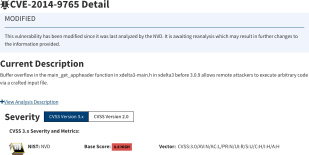
\includegraphics[width=\framewidth]{media/cve-2014-summary}
  }
  \only<2>{
  \includegraphics[width=\framewidth]{media/cve-2014-ref}
  }
  \only<3>{
  \includegraphics[width=\framewidth]{media/xdelta-commit}
  }
\end{frame}

\begin{frame}[fragile]\frametitle{The bug}
  \begin{lstlisting}[numbers=left, language=C, emph={parsed}, emphstyle={\alert}, emph={[2]place}, emphstyle={[2]\color{brown!60!black}}]
xd3_get_appheader (stream, & apphead, & appheadsz);

char *start = (char*)apphead;
char *slash;
int   place = 0;
char *parsed[4];
memset (parsed, 0, sizeof (parsed));

while ((slash = strchr (start, '/')) != NULL) {
  *slash = 0;
  parsed[place++] = start;
  start = slash + 1;
}
  \end{lstlisting}
\end{frame}

\begin{frame}[label=current]\frametitle{Existing datasets}
  \small
  % diversity % label precision
  % size
  % naturalness
  \rowcolors[]{1}{}{lightgray}
  \begin{tabular}{rrrll}
    \toprule
    name & code source & label source & label quality & size \\
    \midrule
    Juliet (SATE IV) & synthetic & human & + & +\\
    SARD\footnote{\scriptsize{\url{https://samate.nist.gov/SARD/}}} & mixed & human & + & + \\
    Draper\footnote{\fullcite{russell_automated_2018}} & GitHub,Debian & static analyser & - & +  \\
    Devign\footnote{\fullcite{zhou_devign_2019}} & FFmpeg,Qemu & human & + & - \\
    ReVeal\footnote{\fullcite{chakraborty_deep_2020}} & Debian,Chrome & NVD patch & \textasciitilde{} & \textasciitilde{} \\
    \bottomrule
  \end{tabular}

  \begin{tikzpicture}[overlay]
    \draw[->,thick] (12.25,2.6) -- node[align=left, right]{natural-\\ness} (12.25,0.2);

  \end{tikzpicture}

\end{frame}

\begin{frame}[label=current]\frametitle{Challenge 1: compilation}
  \begin{tikzpicture}
  \def\lwidth{0.1pt};
  \begin{scope}[local bounding box=samples]
    \def\corner{0.15in};
    \def\cornerradius{0.02in};
    \def\h{1.7cm};
    \def\w{2cm};
    \foreach \i in {0,1,2} {
    \coordinate (nw) at ($(-0.05in*\i,-0.06in*\i)$);
    \coordinate (ne0) at ($(nw) + (\w, 0)$);
    \coordinate (ne1) at ($(ne0) - (\corner, 0)$);
    \coordinate (ne2) at ($(ne0) - (0, \corner)$);
    \coordinate (se) at ($(ne0) + (0, -\h)$);
    \filldraw [-, line width = \lwidth, fill=white] (nw) -- (ne1) -- (ne2)
    [rounded corners=\cornerradius]--(se) -- (nw|-se) -- cycle;
    \draw [-, line width = \lwidth] (ne1) [rounded corners=\cornerradius]-- (ne1|-ne2) -- (ne2);
    }
    \node[anchor=north west,node distance=0] at (-0.05in,-0.8) {Samples};
  \end{scope}

  \matrix[ right=6em of samples, column sep=0pt, ampersand replacement=\&] (debian) {
    \node[anchor=center] {\includegraphics[width=2em]{media/debian-openlogo-nd}}; \& \node[anchor=base, name=deb-pkg, outer sep=0.5em]{Deb. Package}; \\
  };

  \matrix[above={3em of debian}, column sep=0pt, ampersand replacement=\&] (trace) {
    \node[anchor=center] {
\includegraphics[width=2em]{media/glass}}; \& \node[anchor=base, yshift=-0.15em]{Build Trace}; \\
  };

  \matrix[above right={2em and 6em of trace.center}, column sep=0pt, ampersand replacement=\&] (compy) {
    \node[anchor=center] {\includegraphics[width=4em]{media/llvm-logo-deriv1}}; \& \node[anchor=base, yshift=-0.15em]{ComPy-Learn}; \\
  };

  \draw[thick]
    (samples) edge[bend right=20, in=-120, out=-45, ->] node[above=0.6em, sloped]{\small\emph{1. link via CVE}} (deb-pkg.center |- deb-pkg.south)
    (deb-pkg) edge[->] node[right=0.6em]{\small\emph{2. record build commands}} (deb-pkg |- trace.south)
    (deb-pkg |- trace.north) edge[out=90, in=180, ->] node[left=0.8em]{\small\emph{3. extract compile flags}} (compy)
  ;

\end{tikzpicture}
%%% Local Variables:
%%% TeX-master: "../scratch.tex"
%%% End:

\end{frame}

\begin{frame}[label=current]\frametitle{Challenge 1: compilation}
  \begin{center}
  \begin{tikzpicture}
    \begin{scope}[local bounding box=pie]
      \pie[sum=auto, text=legend, color={pGreen, pYellow, pGray}]{
        910/compiled,
        70/preprocessed,
        432/failed
      };
    \end{scope}

    \node[anchor=south east, above right=5em, yshift=1.5em, text width=8em] at (pie.center) {1412 total files\\{\scriptsize from 698 package instances}};

  \end{tikzpicture}
  \end{center}
\end{frame}

% ReVeal
% Devign
% Draper
% SARD/SATE
%

\begin{frame}\frametitle{Challenge 2: dataset is noisy}
  \begin{center}
  \includegraphics[height=0.7\textheight]{media/reveal-unbalanced-crop}
  \end{center}
\end{frame}

\begin{frame}\frametitle{Challenge 2: dataset is noisy}
  \includegraphics[width=\textwidth]{media/libav-big-commit}
\end{frame}

\section{Results}

\begin{frame}[label=current]\frametitle{Experiments}
  \textbf{Hardware (ZIH HPC cluster)}
  \begin{itemize}
    \item CPU: IBM Power9 CPU (2.80 GHz, 3.10GHz boost)
    \item GPU: NVIDIA VOLTA V100 with 32GB HBM2
    \item RAM: 16GB
  \end{itemize}

  \vspace{1em}

  \textbf{Parameters}
  \begin{itemize}
    \item Hidden dimension: 32
    \item GGNN timesteps: 3-1-3-1
    \item Sandwich layers: RNN GGNN RNN GGNN RNN
  \end{itemize}
\end{frame}


\begin{frame}\frametitle{Accuracy for vulnerable function pairs}
  \includegraphics[width=\framewidth]{media/plot-acc-paired}
\end{frame}

\begin{frame}\frametitle{Detecting patched vs never patched functions}
  \includegraphics[width=\framewidth]{media/plot-acc-exclusive}
\end{frame}

\begin{frame}[t, label=current]\frametitle{Future directions}
  \begin{tabular}{p{0.4\framewidth}@{\hskip 3em}p{0.4\framewidth}}
      \textbf{model architecture} & \textbf{dataset} \\
      \begin{itemize}
        \itemsep0.6em
        \item handle identifiers
        \item include representations of called functions
        \item simplify graph
        \item predict location of bug
      \end{itemize} &
      \begin{itemize}
        \itemsep0.6em
        \item more heuristics for compiling
        \item better filtering
        \item alternative sources: OSS-Fuzz\footnote{\url{https://google.github.io/oss-fuzz/}}
        \item fuzzy parsing: Joern\footnote{\url{https://joern.io/}}
      \end{itemize}
    \\
  \end{tabular}
\end{frame}

\begin{frame}\frametitle{Summary}
  \begin{columns}
    \begin{column}{0.5\textwidth}
      \vspace{-2.5em}
      \begin{enumerate}
        \itemsep1em
        \item implemented sandwich model using compy learn
        \item no model able to generalize on real world data
        \item real world data is hard to find, need better datasets first
      \end{enumerate}
    \end{column}
    \begin{column}{0.5\textwidth}
      \uncover<2>{
      \includegraphics[width=0.8\textwidth]{media/bug-captcha}
      }
    \end{column}
  \end{columns}
\end{frame}

\appendix

\begin{frame}[allowframebreaks]{References}
  \printbibliography
\end{frame}


\end{document}
